\documentclass[a4paper]{article}
\usepackage[utf8]{inputenc}
\usepackage{listings}
\usepackage{anysize}
\usepackage{pgfplots}
\usepackage{graphicx}
\title{\vspace{-2.0cm}Software Security A.A.2018-2019\\
Individual Project 1}
\author{Serena Ferracci 1649134}
\date{October 2018}
\marginsize{3cm}{3cm}{1cm}{1cm}


\begin{document}

\maketitle
\section*{Splint}
Splint is a tool for statically checking C programs for security vulnerabilities 
and programming mistakes.  Splint does many of the traditional checks 
including unused declarations, type inconsistencies, use before definition, 
unreachable code, ignored return values, execution paths with no return, likely 
infinite loops, and fall through cases.  More powerful checks are made possible 
by additional information given in source code annotations.  Annotations are 
stylized comments that document assumptions about functions, variables, 
parameters and types.  
The program can add these annotations to the code to for a better result and doing that he will understand
better the code and what is going on, so he can also spot simpler the possible errors in the code.
Moreover, users can define new annotations and an associated check to extend Splint’s checking ability.
The negative side of these annotations: if a user want to analyze a file or a project that is already written
it is not so easy to put annotations, especially
when the file is quite big.

Another important down side is that the tool gives a lot of false positives or warnings 
that might be unimportant, as an example: coding style recommendations. 
To work around this problem, the tool offers the possibility 
to customize the showed result selecting what types of errors are reported using 
command line flags and stylized comments in the code.

In conclusion, Splint is a great tool for finding errors in all areas of an application, but if a
programmer is specifically looking for security bugs, Splint can not compete with
the other tools. It is recommended that
Splint be used along side of another scanner like RATS or Flawfinder, which
would re-enforce the search for security vulnerabilities.

\subsection*{File A}
\begin{figure}[h!]
    \centering
    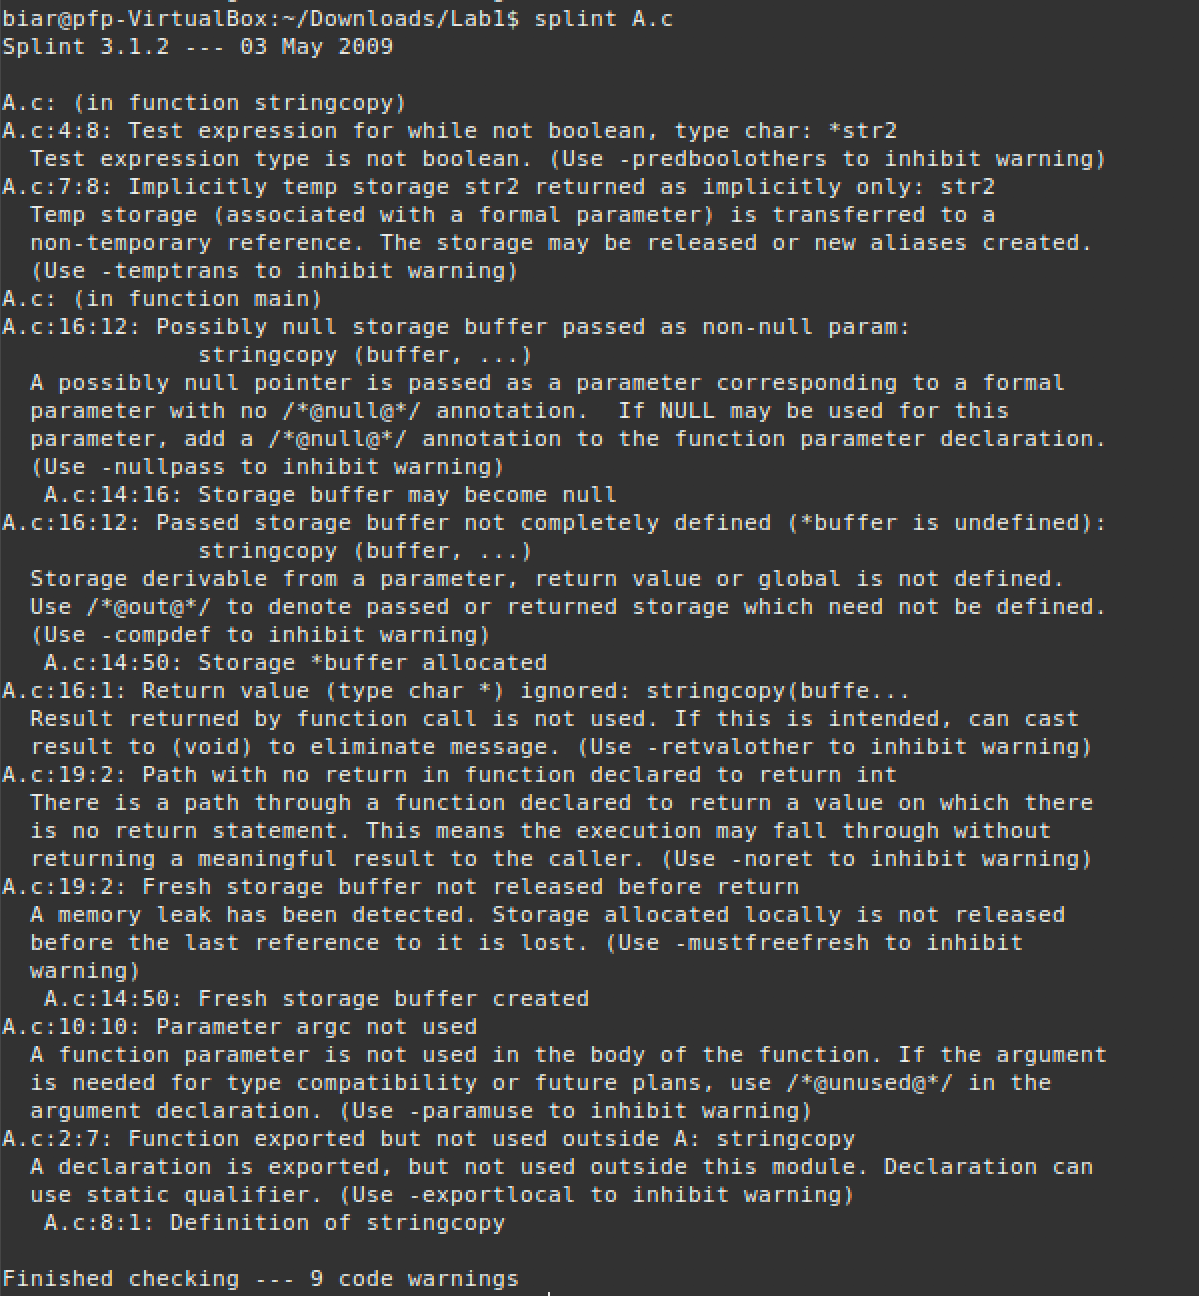
\includegraphics[width=0.4\linewidth]{screen-A}\quad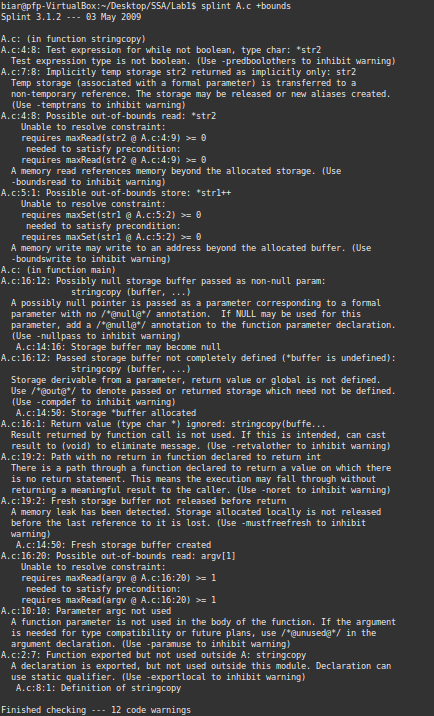
\includegraphics[width=0.4\linewidth]{A-bound}
    \caption{Splint A.c without and with bounds warnings}
\end{figure}

The purpose of the function is to retrieve the string passed to the function through \texttt{argc},
copy the string into a buffer and then print the buffer to the user.

The warnings showed by Splint are 9 and some of them are real vulnerabilities, others are 
not so important. The warnings are:
\begin{itemize}
    \item \texttt{Test expression for while not boolean}. This warning is not important,
        Splint does not recognize implicit test expressions as valid ones.
        To solve the warning, it is added an explicit test. The function checks is the analyzed
        character is a string terminator.
    \item \texttt{Implicitly temp storage str2 returned as implicitly only}. The auxiliary function 
        return \texttt{str2} that was passed as parameter. Splint sees the variable as a temporal one 
        and so informs the user that the storage may be released or new aliases created for str2.
        There are two possible solution: 
        \begin{itemize}
            \item mark the str2 variable as \texttt{/*@returned@*/}.
            Splint assumes the result of \texttt{stringcopy} is the same storage as its second
            parameter. No error is reported, since the only
            storage is then transferred through the return value.
            \item since the returned value is not used in the main function, it is possible
            to change the return value to void and, in this way, it does not return anything. The logics of the 
            function does not change, it still perform the copy.
        \end{itemize}
    \item \texttt{Possibly null storage buffer passed as non-null param}. The parameter \texttt{buffer}
        passed to the \texttt{stringcopy} function can be NULL. In fact after the allocation, there is not
        a check to verify the correct execution of the \texttt{malloc} function.
        To solve the warning, it is check on the return value of the \texttt{malloc} function.
    \item \texttt{Passed storage buffer not completely defined}. The first parameter passed to 
        to \texttt{stringcopy} is just allocated in main, so it must be marked as \texttt{/*@out@*/}
        to denote passed storage which need not be defined.

    \item \texttt{Return value (type char *) ignored}: The resolution of this warning depends on how 
        the warning on str2 has been salved. If the function is declared as void, this warning 
        it is solved implicitly. Otherwise, the return value of \texttt{stringcopy} is stored in a variable.
        The presence of this variable will cause another warning, the storage should be released 
        before the return statement. Since the variable is another pointer to the memory area pointed by
        str2, that is \texttt{argv[1]}, there is no need to free the area. So, it can be considered 
        a false positive.

    \item \texttt{}{Path with no return}. In the main function is missing the return statement. To
        solve the warning it is added \texttt{return 0} at the end of the main function.

    \item \texttt{Fresh storage buffer not released before return}. The warning refers to the variable 
        \texttt{buffer} that is allocated using malloc, but it is not released before the return statement.
        For this, \texttt{free(buffer)} is added in the main function before the return.

    \item \texttt{Parameter argc not used}. The parameter argc is passed to the main function, but
        it is not used. The parameter contains the number of input is passed by the user, so it is useful
        to check if argv contains at least a value, that will be the one used by the function. 
    
    \item \texttt{Function exported but not used outside}. Since the function is not used outside, it
        is declared as static. The access to static functions is restricted to the file where they are declared.
\end{itemize}

Using the flag \texttt{+bounds} the warnings are 12. The 3 additional warnings are: 
\begin{itemize}
    \item \texttt{Possible out-of-bounds read: argv[1]}. The warning is salved adding the annotation: 
        \texttt{/*@requires maxRead(argv) >= 1 $\wedge$ maxRead(argv[1]) >= 0 @*/}. A requires clause specifies a predicate
        that must be true at a call site; when checking a function implementation Splint assumes the
        constraints given in its requires clauses are true at function entry.
    \item \texttt{Possible out-of-bounds read: *str2} and \texttt{Possible out-of-bounds store: *str1++}.
        The annotation used to salve the two warnings is \texttt{/*@requires maxRead(str2) >= 0 $\wedge$ maxSet(str1) >= 0@*/}. 
        So as to ensure that the two variables have at least a dimension greater or equal than 0.
\end{itemize}


\subsection*{File B}

To the original file, a basic main function is added in order to compile and 
execute the file. In this way it is possible to understand better what the 
executable do and what are the vulnerabilities. The main function is only used to 
open an existing text file, defined to text the executable, and to call the 
original function, \texttt{func}, passing as parameter the file descriptor of the 
file just opened. After the call, the main function close the text file and return.

\begin{figure}[h!]
    \centering
    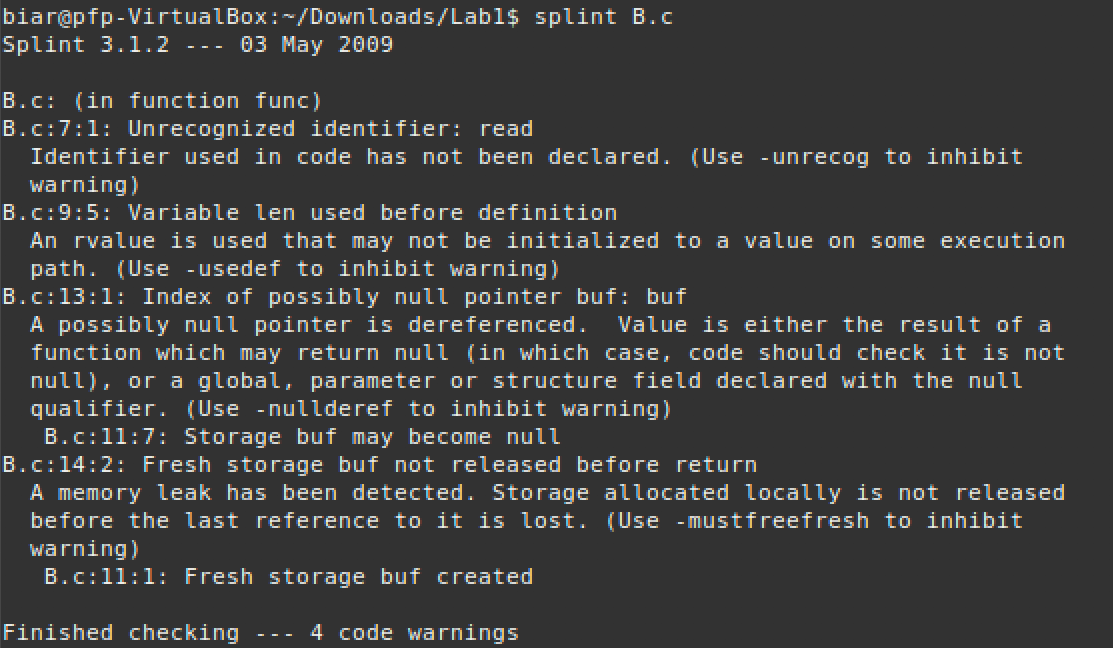
\includegraphics[width=0.47\linewidth]{screen-B}\quad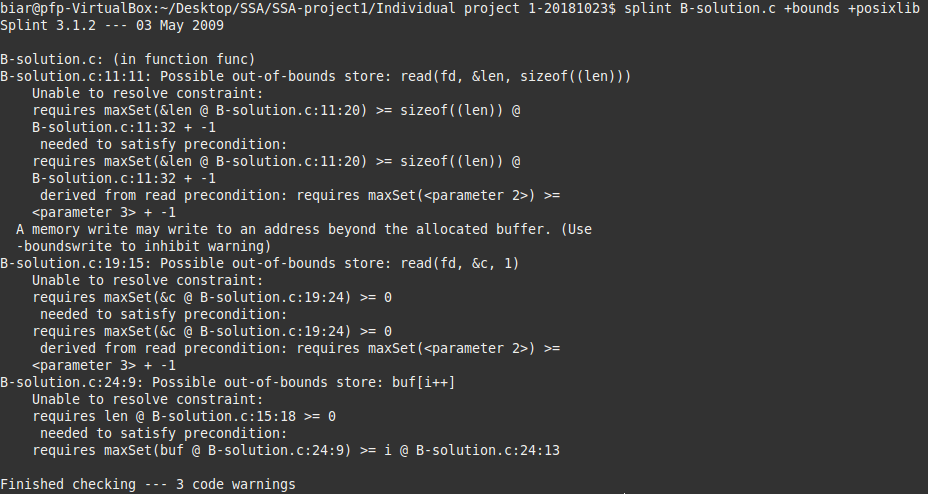
\includegraphics[width=0.47\linewidth]{B-bound}
    \caption{Splint B.c with and without flags}
\end{figure}

The purpose of the function \texttt{func} is to read on a file an integer, that 
will be used to define the size of a buffer, and read 

\subsection*{File C}
\begin{figure}[h!]
    \centering
    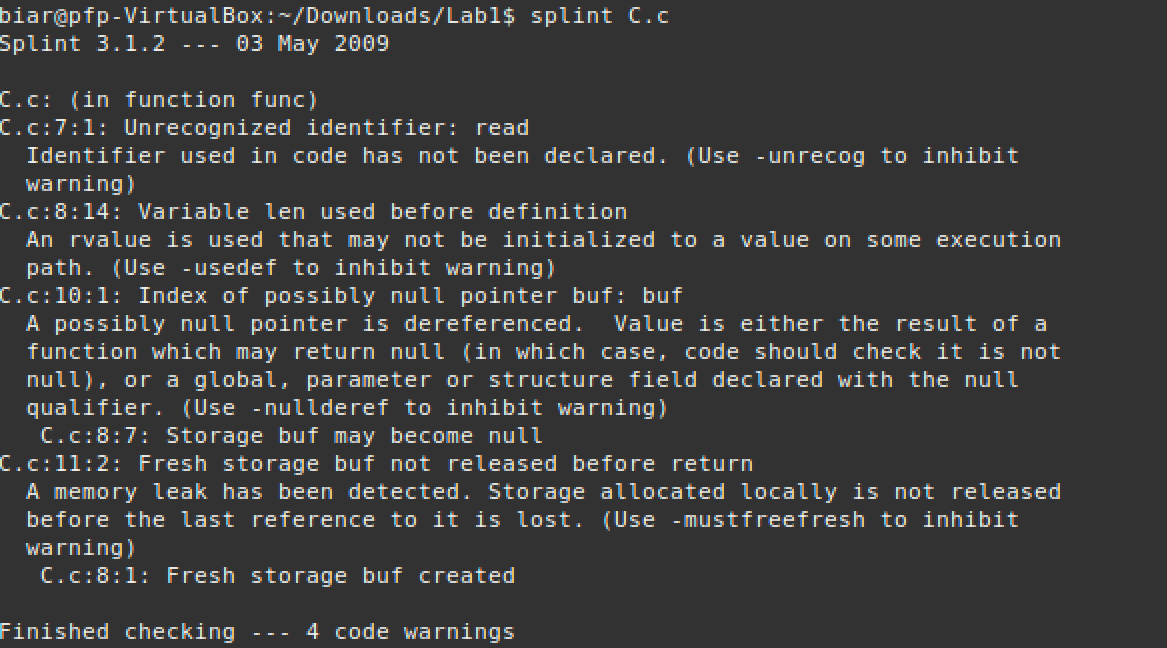
\includegraphics[width=0.6\linewidth]{screen-C}
    \caption{Splint B.c}
\end{figure}

\section*{FlawFinder}

Flawfinder is a simple yet efficient ad quick tool that scans your C/C++ source 
code for calls to typical vulnerable library functions. It was developed by 
David Wheeler external link, a renowned security expert. It is run from the 
command line. Its output can easily be customized using specific command-line options. 
It is possible to call Flawfinder on a folder and it will analyze all the files
present in it, but this analysis should be done only to have a general idea on the folder.
The result of the analysis is a list of possible vulnerabilities divided by levels, the tool
show first the riskiest ones.
After the fist analysis, the user should call Flawfinder on each single file, possibly starting 
from the one with the riskier vulnerabilities.

Flawfinder has some pros and cons. Flawfinder works by doing simple
lexical tokenization (skipping comments and correctly tokenizing strings), 
looking for token matches to the
database, so the tool is base on a black list. 
Flawfinder then examines the text of the function parameters to estimate risk.
Unlike tools such as splint, gcc’s warning flags, and clang, 
flawfinder does not use or have access to information
about control flow, data flow, or data types when searching 
for potential vulnerabilities or estimating
the level of risk. Thus, flawfinder will necessarily produce many 
false positives for vulnerabilities and fail
to report many vulnerabilities. On the other hand, 
flawfinder can find vulnerabilities in programs that cannot
be built or cannot be linked. It can often work with programs 
that cannot even be compiled (at least by
the reviewer’s tools). Flawfinder also doesn’t get as confused 
by macro definitions and other oddities that
more sophisticated tools have trouble with. Flawfinder can 
also be useful as a simple introduction to static
analysis tools in general, since it is easy to start using and easy to understand.

\subsection*{File A}
\begin{figure}[h!]
    \centering
    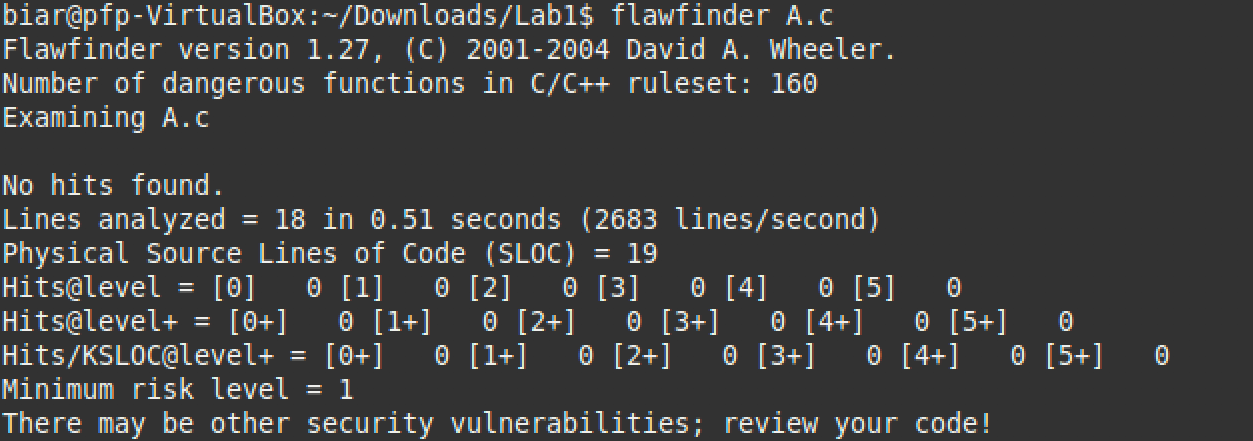
\includegraphics[width=0.48\linewidth]{A-f}\quad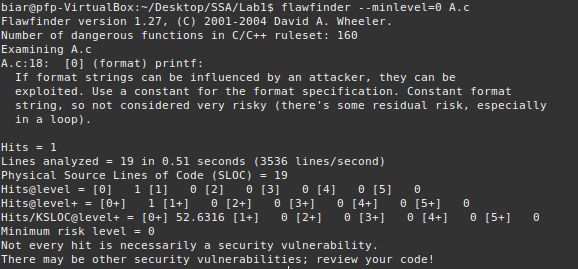
\includegraphics[width=0.48\linewidth]{min-A}
    \caption{FlawFinder A.c minlevel=1 and minlevel=0}
\end{figure}

There is only one hit that suggest to use a constant for the format specification, otherwise an 
attacker could influence the format string. This can be considered a false positive since or
just a suggestion derived from the simple presence of \texttt{printf}, since it is already used 
a constant format.
\bigskip

\begin{figure}[h!]
    \centering
    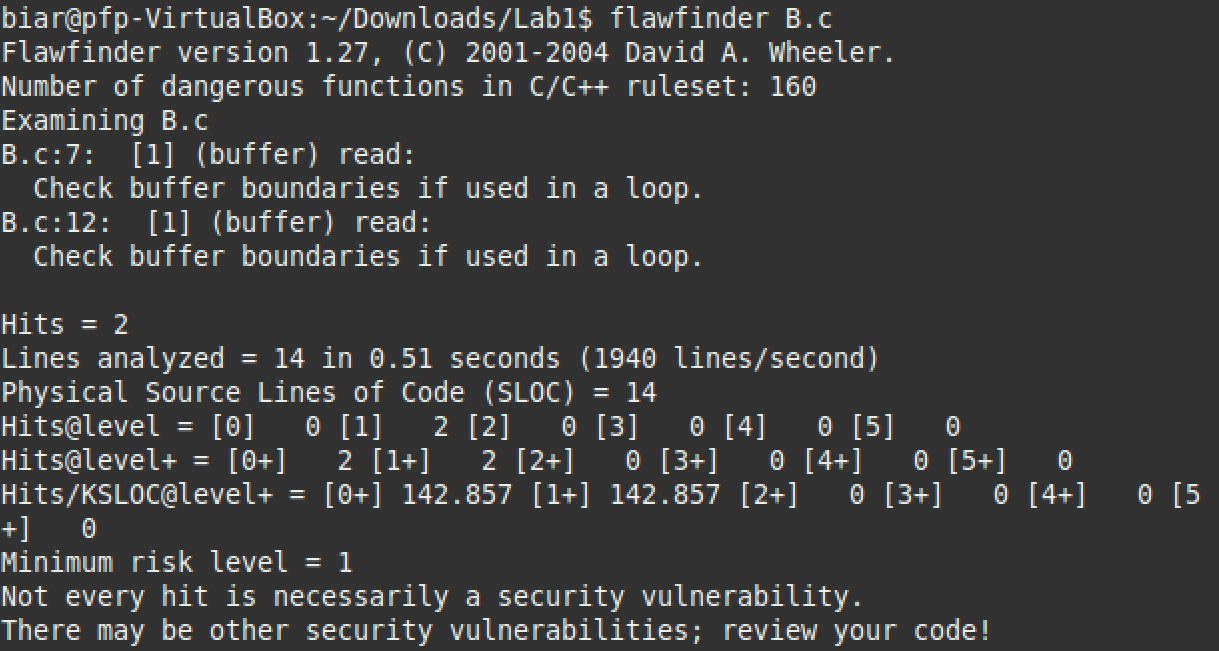
\includegraphics[width=0.6\linewidth]{B-f}
    \caption{FlawFinder B.c}
\end{figure}

\begin{figure}[h!]
    \centering
    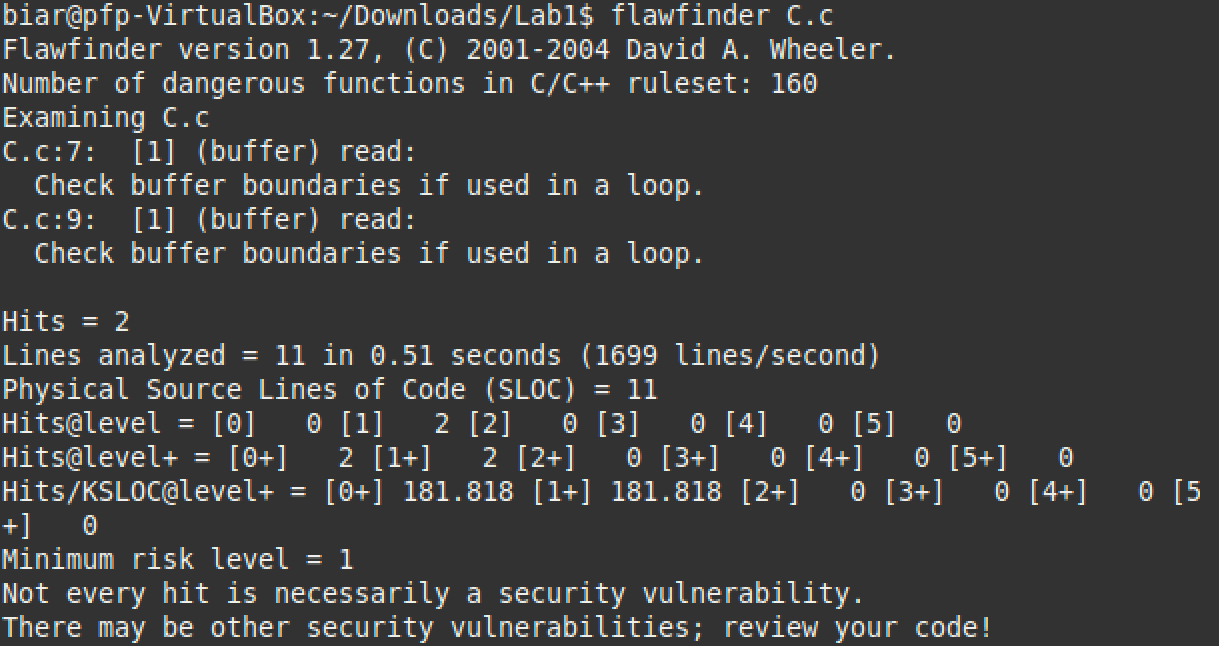
\includegraphics[width=0.6\linewidth]{C-f}
    \caption{FlawFinder B.c}
\end{figure}

\end{document}